%%\documentclass[aip,jcp]{revtex4-1}
\documentclass[aip
, pra
, showpacs
, aps
, twocolumn
%, onecolumn
, groupedaddress
, floatfix
%, preprint
]{revtex4}
%]{revtex4-1}
\usepackage{graphicx, amsbsy, bm, dcolumn, amsmath}

\newcommand{\etal}{{\em et~al.\/}}
\newcommand{\beq}{\begin{equation}}
\newcommand{\eeq}{\end{equation}}
\newcommand{\barr}{\begin{array}}
\newcommand{\earr}{\end{array}}
\newcommand{\vecr}{{\bf r}}
\newcommand{\dd}{\mbox{d}}
\newcommand{\dr}{\mbox{d} r}
\newcommand{\vare}{\varepsilon}
\newcommand{\calN}{{\cal N}}
\newcommand{\di}{_{\mbox{\tiny{di}}}}
\newcommand{\ex}{_{\mbox{\tiny{ex}}}}



\newcommand{\isum}%
{\mathop{\hbox{$\displaystyle\sum\kern-13.2pt\int\kern1.5pt$}}}

\begin{document}

\title {$J$-matrix calculation of electron-helium $S$-wave scattering. II. Beyond the frozen-core model}

\author{Dmitry A. Konovalov}
\affiliation{ARC Centre for Antimatter-Matter Studies}
\affiliation{Discipline of Information Technology, School of Business, James Cook University, Townsville, Queensland 4811, Australia}

\author{Dmitry V. Fursa}
\affiliation{ARC Centre for Antimatter-Matter Studies,
Curtin University, GPO Box U1987, Perth, Western Australia 6845, Australia}

\author{Igor Bray}
\affiliation{ARC Centre for Antimatter-Matter Studies,
Curtin University, GPO Box U1987, Perth, Western Australia 6845, Australia}



\date{\today}

\begin{abstract}
In the preceding paper  [Konovalov {\em et. al.} Phys. Rev. A {\bf 84}, 032707 (2011)] we used
the $J$-matrix method to solve  the $S$-wave $e$-He scattering problem within the frozen-core model of helium.
In the present work we go beyond the frozen-core model and adopt a general configuration-interaction description of helium (within $S$-wave model).
As a result a more accurate description of helium target states is achieved that allowed us to obtain highly
accurate numerical solutions of the $e$-He scattering problem
for the elastic, $2^{1,3}S$, $3^{1,3}S$ excitation and total ionization cross sections.
At energies above the ionization threshold some minor pseudo-resonance behavior is still evident despite the large bases used.
The $J$-matrix results are confirmed by the corresponding convergent-close-coupling calculations creating a challenging benchmark
for any current or future {\it ab initio} electron-atom scattering methods.



\end{abstract}

\pacs{34.80.Dp} %34.80.Dp	Atomic excitation and ionization
\maketitle



\section{INTRODUCTION}


This study focuses on the $S$-wave $e$-He ($e$-He($S$)) scattering model,
where the target helium atom is in its ground state before the electron impact,
and where only the partial wave with zero angular momentum ($l=0$) is retained in all calculations
and partial-wave expansions.
The $S$-wave models have proven to be a very productive testing ground for {\it ab initio} scattering theories,
see \cite{T62,HY74p1209,P78,P80,P81,CO84,BS92p53,BST93,KM94pL407,IDHF95,PS96,JS02,JS00l,BRIM99,S99l,MHR02,BS04,Frapiccini10} for the $S$-wave $e$-H scattering ($e$-H($S$))
and \cite{DHIF94,PMR99,PBFS02,PNBFS04,HMR05R,HMR05,BS10p022715,BS10p022716,KFB11} for  the $e$-He($S$) problem.
The main attraction of the $S$-wave models is that they retain most of the physics complexities of the full
scattering problems while reduce the problems computationally.
Furthermore it is generally expected that if a theoretical method solves a $S$-wave model, then
the remaining partial waves could be solved with additional computational resources,
see for example the convergent-close-coupling (CCC) \cite{FB95},
$R$-matrix (RM) \cite{FLRS94b, PhysRevA.54.R998, SMC2006}
and $J$-matrix (JM) \cite{KM94pL741,KM95pL139} methods.


The main goal of this study is to provide high accuracy $e$-He($S$) cross sections highlighting resonant features of the cross sections where applicable.
The need for such benchmark calculations is evident from the existing {\em ab initio} attempts to solve the $e$-He($S$) problem.
Reviewing in reverse chronological order, in 2010, \citet{BS10p022715} developed a four-body propagating exterior scaling (PECS) method and reported results claiming to achieve "benchmark" level of accuracy.
However none of their cross sections, including elastic and $2^{1,3}S$ excitation cross sections,
displayed resonances at the accuracy level achieved for the $e$-H($S$) problem \cite{P78}.
In 2005, \citet{HMR05} reported results using
time-dependent exterior complex scaling (TD-ECS), which also omitted description of resonance behavior of the cross sections.
In 2002 and 2004, the CCC method \cite{PBFS02,PNBFS04} did not examine the resonance regions with a sufficiently fine energy grid.
This is now corrected to some extent when in 2011 \citet{KFB11} reported the CCC and JM {\em frozen-core}
(FC) results clearly showing the resonances in the elastic and $n=2$ ($2^1S$ and $2^3S$) excitation cross sections.
As far as we are aware, the RM method \cite{FLRS94b, SMC2006}, which is most suited to the study of resonances,
has never reported its results for the $e$-He($S$) problem.
In summary, while the three most advanced theoretical methods (PECS, TD-ECS, CCC) are in good qualitative or overall agreement with each other,
in many specific cases their results differ by as much as 10-20\% \cite{BS10p022715,HMR05}.
These discrepancies together with the unexplored resonance features of the model,
provides the motivation for the present study.


The stated goal is achieved by combining advantages of the CCC and JM methods,
where the latter has been recently revised \cite{KFB11} by merging it with the Fano's multi-configuration interaction matrix elements \cite{Fano65}.
The CCC method is able to solve the scattering problem very accurately via the Lippmann-Schwinger equation \cite{BS92p6995}.
However, it is not practical to run the CCC method for each of the many thousands of impact energy points required for the final benchmark results.
On the other hand, the JM method is very efficient \cite{HY74p1201,BR76p1491} in calculating a vast number of energy points
but numerical-convergence properties of the JM method remain largely unknown.
The JM and CCC methods are implemented independently and use completely different approaches to solve the scattering equations.
Therefore, the CCC and JM methods were used to cross-verify that their results are convergent within their own numerical parameters at key energy points.
See \cite{JMatrixWebsite} for information on availability of the results and source code.


\begin{figure*}[htb]
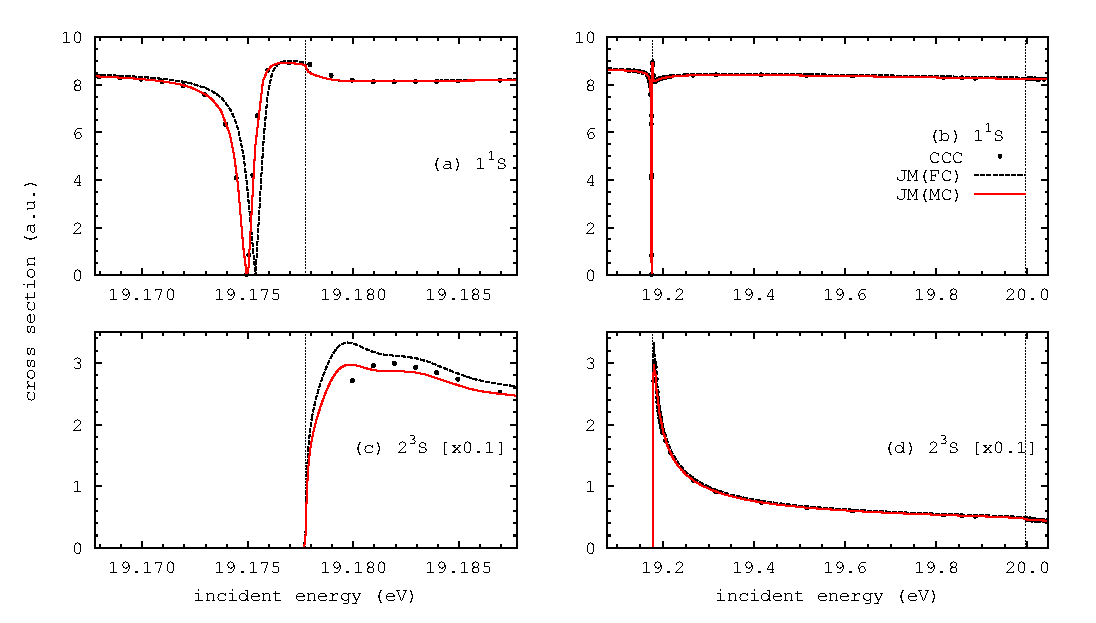
\includegraphics[scale=1]{fig1.ps}
\caption{(Color online) Elastic ($1^1S$) and
$2^3S$ single-excitation $e$-He $S$-wave cross sections between and around $2^3S$ and $2^1S$ thresholds shown by vertical dashed lines.
Sub-figures (a) and (c) zoom in on the $2^3S$ excitation threshold (Table~\ref{Tab_ENGS}).
JM(FC) ($N_c=1$, $N_t=30$), JM(MC) ($N_c=7$, $N_t=30$) and CCC ($N_c=3$, $N_t=30$) results  were shifted to the right by 0.17747~eV, 0.0018~eV
and 0.01594~eV (Table~\ref{Tab_ENGS}), respectively.
}
\label{Fig_1}
\end{figure*}


\begin{figure}[htb]
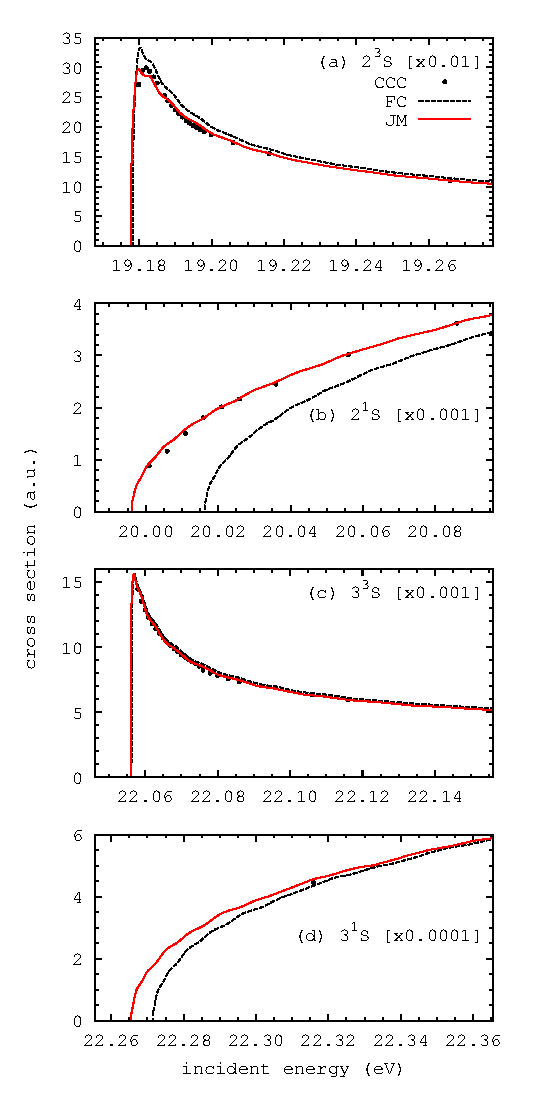
\includegraphics[scale=1]{fig2.ps}
\caption{(Color online) The same as in Fig.~\ref{Fig_1} but with added $2^1S$ excitation cross section, and
for incident energies between and around $2^1S$ and $3^3S$ thresholds shown by vertical dashed lines.
}
\label{Fig_2}
\end{figure}


\begin{figure*}[htb]
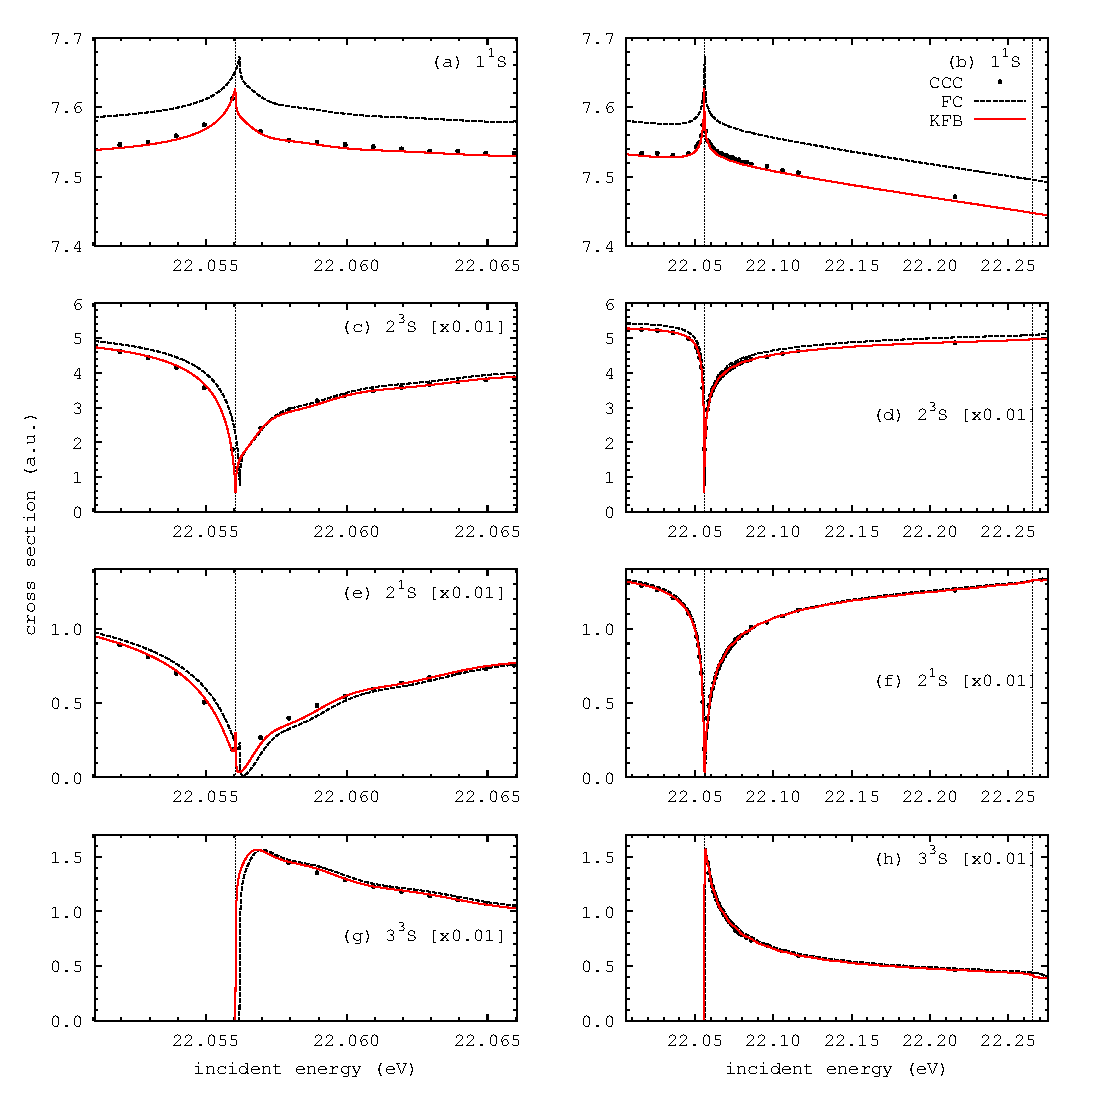
\includegraphics[scale=1]{fig3.ps}
\caption{(Color online)
The same as in Fig.~\ref{Fig_2} but with added $3^3S$ excitation cross section, and
between and around the $3^3S$ and $3^1S$ thresholds shown by vertical dashed lines.
Sub-figures (a), (c), (e) and (g) zoom in on the $3^3S$ excitation threshold (Table~\ref{Tab_ENGS}).
TEST denotes the JM(FC) calculation with $N_c=1$, $N_t=20$ and $N=21$.
}
\label{Fig_3}
\end{figure*}

\begin{figure}[htb]
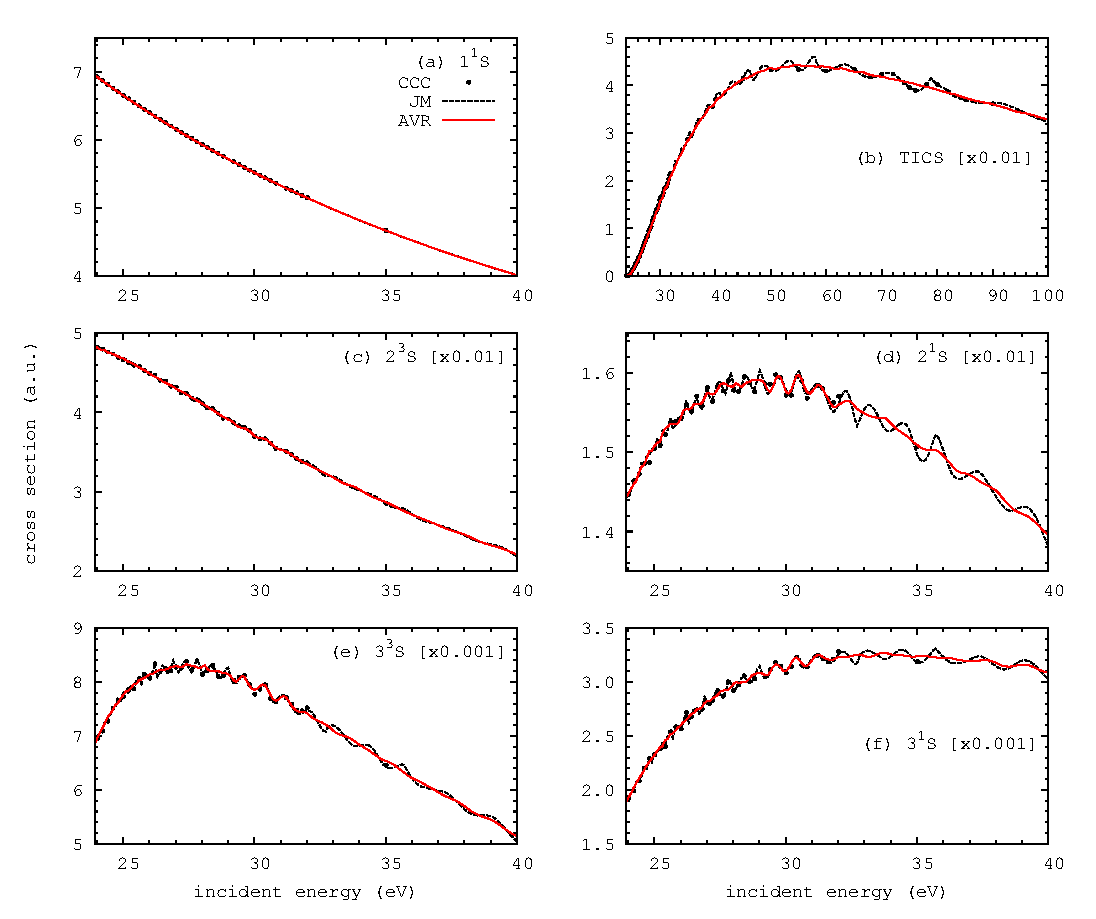
\includegraphics[scale=1]{fig4.ps}
\caption{(Color online)
The same as in Fig.~\ref{Fig_3} but with added $3^1S$ excitation cross section
between the $3^3S$ and ionization thresholds (23.92~eV, Table~\ref{Tab_ENGS}).
The $3^1S$, $4^{3,1}S$, ..., $7^{3,1}S$ excitation thresholds (Table~\ref{Tab_ENGS})
are shown by vertical dashed lines (from left to right).
}
\label{Fig_4}
\end{figure}


\begin{figure*}[htb]
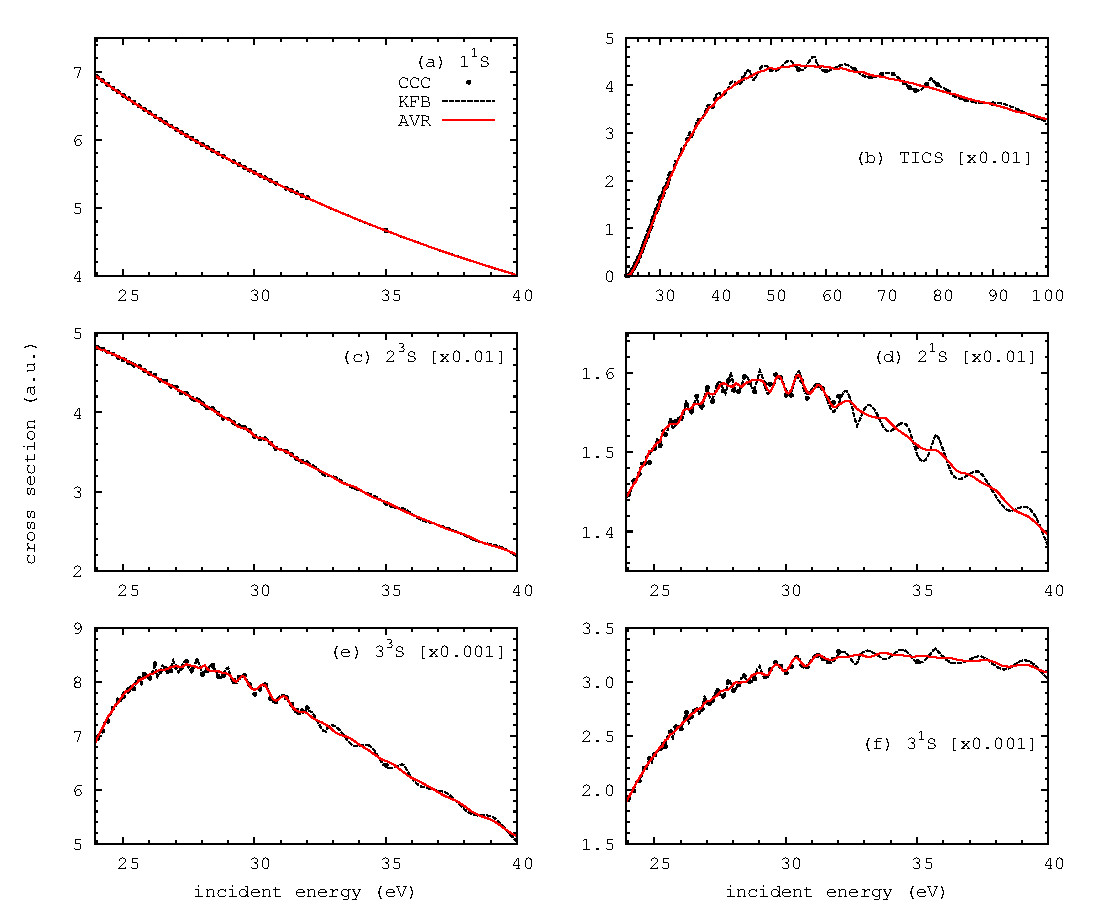
\includegraphics[scale=1]{fig5.ps}
\caption{(Color online)
The same as in Fig.~\ref{Fig_4} but with added total ionization cross section (TICS)
for incident energies above the ionization threshold.
AVR denotes averaged JM(MC) calculations with $N_c=3$, $25\leq N_t \le 35$ and $N=100$.
Note that in this figure all results are not corrected for the ground energy errors (curves are not shifted).
}
\label{Fig_5}
\end{figure*}


\begin{table}[htb]
\caption{\label{Tab_ENGS}
Energy levels (a.u.) and excitation thresholds (eV) of the first nine bound states of helium in the
$S$-wave model.
}
\begin{ruledtabular}
%\begin{tabular}{lcr}
\begin{tabular}{rlll}
Classification & threshold (eV) & Eigenvalues (a.u) & ($N_c$,$N_t$)   \\
\hline
$\mbox{He}(1s^2,^1S)$ & 0  & -2.879 028 57  &  (50,50)   \\ %
            error =   & 0.001 80 & -2.878 962 30   &  (7,30)    \\
            error =   & 0.015 94 & -2.878 442 70   &  (3,30)    \\
            error =   & 0.177 47 & -2.872 506 67   &  (1,30)    \\
\hline
$\mbox{He}(1s2s,^3S)$   & 19.178  & -2.174 264 85  & (50,50) \\  %-2.174 264 856 288154 -2.174264856287701, -2.0684901366080752,
                 &  & -2.174 264 62   &  (7,30)   \\
                &  & -2.174 245 50   &  (1,30)    \\
\hline
$\mbox{He}(1s2s,^1S)$     &  19.996 & -2.144 197 26  &  (50,50) \\ %-2.144 197 258 7 31818,
                          &  & -2.144 191 39   &  (7,30)   \\
                          &   & -2.143 449 32   &  (1,30)    \\
\hline
$\mbox{He}(1s3s,^3S)$     & 22.056  & -2.068 490 07   &  (7,30)   \\
                          &        & -2.068 484 66   &  (1,30)    \\
\hline
$\mbox{He}(1s3s,^1S)$     & 22.266   & -2.060 792 35   & (7,30)    \\
                          &          & -2.060 573 16   &  (1,30)    \\
\hline
$\mbox{He}(1s4s,^3S)$    & 22.928  & -2.036 438 56  &  (7,30)    \\
                         &         & -2.036 436 37   &  (1,30)   \\
\hline
$\mbox{He}(1s4s,^1S)$   &  23.011 & -2.033 392 20 &  (7,30)   \\
                        &         & -2.033 300 71 &  (1,30)   \\
\hline
$\mbox{He}(1s5s,^3S)$   &   23.305  & -2.022 583 69   &  (7,30)    \\
                        &           & -2.022 582 61   &  (1,30)    \\
\hline
$\mbox{He}(1s5s,^1S)$   &  23.346   & -2.021 079 42   &  (7,30)    \\
                        &           & -2.021 033 00   &  (1,30)    \\
\hline
$\mbox{He}^+(1s)$       &  23.920 & -2 	 &    Ionization \\

%nc50 -2.8790285691206896, -2.1441972587317903, -2.0607940375466596, -2.033378552299511, -2.0197845131866514,
%nc50 -2.8790285691204813, -2.144197258731818, -2.060794037546691, -2.0333785522995016, -2.019784513192403,
%-2.174264856288154, -2.0684901366081845, -2.0364341783161515, -2.021798838036517,

%nc10   -2.878976298682523, -2.1441926558786752, -2.0607927208274255, -2.0333923539473497,
% -2.1742647128049755, -2.0684900966824507, -2.036438571423033,

%nc7 -2.8789623026211353, -2.1441913928180427, -2.0607923564616435, -2.0333922030334937, -2.0210794228323463,
% -2.1742646178307643, -2.068490069685457, -2.036438559573639, -2.022583694613397,

%nc1 -2.872506672905663, -2.143449321021511, -2.06057316103011, -2.033300705504141, -2.0210330065059448,
% -2.1742455043163393, -2.0684846598208337, -2.0364363721136964, -2.022582608219962,

\end{tabular}
\end{ruledtabular}
\end{table}



\section{THEORY}

The JM method \cite{JMatrix2008,HY74p1201,BR76p1491} is a general method for solving a wide range of scattering problems.
In this study, we continue to develop the version of the JM method that
was previously applied to the $e$-H($S$) \cite{KB10p022708}  and $e$-He($S$) \cite{KFB11} scattering problems.
In application of the frozen-core version JM(FC)
to $e$-He($S$) \cite{KFB11} scattering one electron was always in the $1s$ state of He$^+$.
The following three sets of functions were deployed: target basis, JM functions, and Laguerre basis.
{\em Target basis} is a set of $N_t$ orthonormal radial functions $\{P_n(r)\}_{n=1}^{N_t}$,
where $P_n(r)$ is used as the radial component of the $n$'th subshell wave function
when building one- or many-electron wave functions as per the Fano's procedure \cite{Fano65, KFB11}.
{\em JM functions} are the nonorthogonal Laguerre functions $\{\xi_p(r)\}_{p=0}^\infty$ as per the original JM method
formulation \cite{HY74p1201,BR76p1491},
\beq
\xi_p(r) = x^{l+1} \mbox{e}^{-x /2}
L_p^{2l+1}(x), \ \ \ p = 0, 1, ..., \infty,
\eeq
where $x=\lambda r$, $\lambda$ is Laguerre exponential falloff,
$l = 0$ (for the $S$-model), and $L_p^{\alpha}(x)$ are the associated Laguerre polynomials \cite{abramowitz}.
{\em Laguerre basis} is the set of orthonormal Laguerre functions $\{R_p(r)\}_{p=0}^\infty$,
\beq
R_p(r) = C_p x^{l+1} \mbox{e}^{-x /2}
L_p^{2l+2}(x), \ \ \ p = 0, 1, ..., \infty,
\eeq
\beq
\int_0^\infty dr \ R_p(r) R_{p'}(r) = \delta_{pp'}, \ C_p= \sqrt{\frac{\lambda p!}{ (p+2l+2)!}}.
\eeq
Note that for any fixed $N_t$, both $\{\xi_p(r)\}_{p=0}^{N_t}$ and $\{R_p(r)\}_{p=0}^{N_t}$
span identical functional space \cite{KB10p022708}.


After many numerical experiments, it became apparent that the core excitation functions $\{P_n(r)\}_{n=1}^{N_c}$ should be constructed differently from the rest of the target basis
$\{P_n(r)\}_{n=N_c+1}^{N_t}$. Otherwise, the convergence by $N_c$ is just too slow to be computationally practical.
This is due to the two very different radial scales present in this study.
Accurate account of electron-electron correlations for the ground, $2^3S$ and $2^1S$ states required short-range functions. 
On other hand,  $n>2$ excited states of helium 
resemble $ns$-orbitals of hydrogen and therefore are long-range.
This problem is solved here by using a mix of the short-range $\{R^c_p(r)\}_{p=0}^{N_c-1}$ with $\lambda_c=4$
and long-range $\{R^t_p(r)\}_{p=N_c}^{N_t-1}$ with $\lambda_t=1$  basis sets
when constructing the target basis as follows.


The JM method splits the one-electron radial functional space into {\em inner} $\{\xi_p\}_{p=0}^{N-1}$
and {\em outer} $\{\xi_p\}_{p=N}^\infty$
subsets controlled by the number $N$ of JM functions in the inner subset \cite{HY74p1201,BR76p1491}.
As per functional equivalency \cite{KB10p022708}, in the actual JM calculations the non-orthogonal $\{\xi_p\}_{p=0}^{N-1}$ set is replaced by
the orthogonal $\{R^t_p\}_{p=0}^{N-1}$ set of functions to simplify calculations of relevant matrix elements.
In the JM method, the target basis $\{P_n(r)\}_{n=1}^{N_t}$ must be orthogonal to the outer JM functions $\{\xi_p\}_{p=N}^\infty$, where $N_t<N$.
Let $\lambda \equiv \lambda_t$ and $\hat{I}_t$ be a projection operator into the functional space of $\{R^t_p(r)\}_{p=0}^{N_t-1}$
\beq
\hat{I}_t = \sum_{p=0}^{N_t-1} | R_p^t \rangle \langle R_p^t |,
\label{I_t}
\eeq
then by construction every function from $\{R^t_p(r)\}_{p=0}^{N_t-1}$ and  $\{R^{ct}_p(r)\}_{p=0}^{N_c-1}$
\beq
R^{ct}_p = \hat{I}_t R^{c}_p,
\eeq
is orthogonal to the outer JM functions.
The final target basis $\{P_n(r)\}_{n=1}^{N_t}$ is constructed by making a single orthonormal basis from
$\{R^{ct}_p(r)\}_{p=0}^{N_c-1}$ and $\{R^t_p(r)\}_{p=N_c}^{N_t-1}$
via the Gram-Schmidt process.
Note that in the CCC method the final target basis
$\{P^{\mbox{{\tiny 3C}}}_n(r)\}_{n=1}^{N_t}$ is also built via the Gram-Schmidt process but from
$\{R^{c}_p(r)\}_{p=0}^{N_c-1}$ and $\{R^t_p(r)\}_{p=N_c}^{N_t-1}$ sets, that is, the intermediate $R^{ct}_p$ functions were not required.



Once the target basis $\{P_n(r)\}_{n=1}^{N_t}$ is selected,
the two-electron target-helium wave functions are constructed by allowing first and second helium electrons to occupy the first $N_c$ and $N_t$ radial functions, respectively,
where $N_c$ controls the number of allowed {\em core} excitations with $N_c=1$ being the frozen-core model.
We refer to the multi-core implementation of the JM method as JM(MC).


\section{RESULTS AND DISCUSSION}


The number $N$ is the key JM parameter responsible for the convergence of any implementation of the JM method,
where $N$ is the number of inner JM functions \cite{HY74p1201,BR76p1491}.
That is, the larger the $N$, the more accurate the corresponding JM results are expected to be.
Within the current JM method, maximum value of $N$ is limited to around 100 so that the method remains to be easily accessible
to a wider research community. All JM results presented in this study were calculated on a consumer-grade laptop,
and available in tabular form \cite{JMatrixWebsite}.


The following JM computational parameters were used, see \cite{KB10p022708} for explanation of the parameters:
$\lambda_c=4$, $\lambda_t=1$, $N_t=30$, $N=100$, $\ln(c)=-5 - 2\ln(Z_{\mbox{\tiny{He}}} )$, $Z_{\mbox{\tiny{He}}}=2$, $r_{\max}=500$,
$M_{LCR}=2001$, where the radial grid was between zero and $r_{\max}$, and
$M_{LCR}$ is the number of equally spaced points in the radial LCR grid \cite{KB10p022708}.


The two-electron configurations (in both JM and CCC methods) are constructed by occupying  radial subshells $\{P_n(r)\}_{n=1}^{N_t}$
with all spin-permitted $(n_1s,n_2s)$ and $(1s,n_2's)$ configurations,
where $1 \leq n_1 \leq n_2 \leq N_c$ and $N_c<n_2' \leq N_t$.
The three-electron configurations 
in the JM method are built by adding an extra $n_3s$-electron with
$ n_2 \leq n_3 \leq N$ or $ n_2' \leq n_3 \leq N$ to each of the available two-electron configurations
and keeping only the ones that are permitted by the Pauli exclusion principle and spin-coupling rules,
where remaining inner JM functions are replaced by the {\em transitional} \cite{KFB11} subset $\{P_n(r)\}_{n=N_t+1}^{N} \equiv \{R^t_p(r)\}_{p=N_t}^{N-1}$.


Hereafter JM(FC), JM(MC) and CCC denote results obtained with $N_c=1$, $N_c=7$ and $N_c=3$, respectively.
The ($N_c=7$, $N_t=30$, $N=100$)-combination yields 51 singlet ($^1S$) and 44 triplet ($^3S$) eigenstates of helium, and 8418 eigenstates of He$^-(^2S)$.
We use 27.2116~eV as the atomic unit of energy (or Hartree).


Table~\ref{Tab_ENGS} shows the first nine eigenvalues from diagonalizations of the $S$-wave helium Hamiltonian.
The first three energy levels were also calculated by using
$\{R^{c}_p(r)\}_{p=0}^{N_c-1}$ as the basis for both electrons with $N_c=50$ and $\lambda_c=4$, denoted by $(50,50)$ in Table~\ref{Tab_ENGS},
where the first seven significant digits of the ground state \cite{G94} are reproduced.
This target basis is not computationally practical for the scattering JM calculations but is used here
as a reference from which the $n=1$ and $n=2$ energy errors in $N_c=7$ and $N_c=1$ models are calculated.
Starting from $n=3$, the $(7,30)$-target basis correctly reproduces seven significant digits \cite{DHIF94} of the energy levels.
Selecting $\lambda_c=4$ creates the first target radial function $P_1(r)$ numerically identical to the exact $1s$ state of He$^+$,
when $N_t$ is sufficiently large in Eq.~(\ref{I_t}) as is the case for the used $N_t=30$.
The main improvement of the $(7,30)$-basis over the froze-core case $(1,30)$ is in the ground state of helium,
where the energy errors are about 2~meV and 177~meV, respectively.



Figs.~\ref{Fig_1}-\ref{Fig_5} show nearly exact agreement between the JM(MC) and CCC methods yielding two important conclusions.
First, it confirms that the JM(MC) results are sufficiently convergent by $N$ when solving the scattering equations via the JM method.
Second, both CCC and JM(MC) are convergent by the number of core excitations $N_c$,
where JM(MC) used $N_c=7$ and CCC used $N_c=3$ in Figs.~\ref{Fig_1}-\ref{Fig_4}.
Therefore, $N_c=3$ is actually sufficient for the considered cross sections and energy range, and is used in Fig.~\ref{Fig_5}.


Figs.~\ref{Fig_1}-\ref{Fig_4} show that if the JM(FC) results are shifted (as they are on the figures)
to the right by the FC ground energy error (0.17747~eV, see Table~\ref{Tab_ENGS}),
the JM(FC) and JM(MC) results become very close.
This means that most of the $S$-wave scattering dynamics  is essentially due to
the movement of one electron in the field of unperturbed $1s$ state of He$^+$.
In most cases, the JM(MC) results differ from the JM(FC) results by no more than 10\% (after the shift).
The only exception is Figs.~\ref{Fig_1}(a) and \ref{Fig_1}(c), where the JM(FC) curves were shifted second time to the left by
the JM(FC) $2{^3S}$ energy error (0.53~meV).


In the JM method, many thousand states are obtained from diagonalization of the He$^-$ Hamiltonian,
which approximate the discrete and continuum spectrum of He$^-$.
The standard interpretation of the negative-ion resonances \cite{BC94} attributes the resonance behaviour of cross sections to
the negative-ion states from the ion's discrete spectrum.


Figs.~\ref{Fig_1}(a) and \ref{Fig_1}(c) zoom in onto the negative-ion resonance He$^-(1s(2s)^2,^2S)$ that exists just
below and within 5~meV of the $2^3S$-excitation threshold.
Again, the JM(FC) model fully explains the results, while the JM(MC) model provides the final adjustments to
arrive at the benchmark solution in Figs.~\ref{Fig_1}(a), \ref{Fig_1}(b), and \ref{Fig_1}(d).
Fig.~\ref{Fig_1}(c) exposes the challenging energy region (about 5~meV) just above the $2^3S$ excitation threshold,
where the CCC and JM(MC) results are comparable but slightly different.
Note that the very sharp peak (Fig.~\ref{Fig_1}c) disappears in the real $e$-He scattering
\cite{KM95pL139, HBSBB96} as the He$^-(19.3~eV)$ resonance \cite{Schulz73, BC94, HY99}
moves away from the $2^3S$(19.7~eV) excitation threshold \cite{HBSBB96}.


Figs.~\ref{Fig_2}(c) and \ref{Fig_4}(d) show that the $2^1S$ and $3^1S$ singlet excitations
do not have the resonant behavior at thresholds.
This is interpreted as the absence of
the He$^-(^2S)$ discrete-spectrum states near the singlet thresholds in the $S$-wave model.
Again this is different from the full model, where such He$^-(^2S)$-states do exist yielding sharp
peaks in the $2^1S$ \cite{KM95pL139, HBSBB96} and $3^1S$ \cite{SMC2006} near-threshold cross sections.


Fig.~\ref{Fig_3} reveals very feature-rich  behavior around the triplet $3^3S$  excitation threshold.
The very sharp peak of the $3^3S$ and very sharp dips in the $n=2$ cross sections at the threshold indicate
the existence of a He$^-$ bound state within 1~meV of the  $3^3S$  excitation threshold.
Note the particularly interesting behavior of $2^1S$ cross section presented in
Fig.~\ref{Fig_3}(e), which could only be obtained within the JM method
when both $N_t$ and $N$ are sufficiently large.
The TEST ($N_c=1$, $N_t=20$, $N=21$) line clearly shows how the resonance behavior
is very sensitive to the quality of the relevant He$^-$ wave function.


Fig.~\ref{Fig_4} shows  rich interplay of cross sections between the $3^1S$ and ionization thresholds,
where the He$^-(^2S)$ resonances exist near the corresponding triplet $4^3S$-$7^3S$ helium states.
The magnitude of the resonance peaks/dips is diminishing with $n$ and becomes indistinguishable above $7^3S$.
This is likely due to the He$^-$ states (from He$^-$ diagonalization)
becoming progressively less accurate in describing the true He$^-$ discrete-spectrum states around higher $n$'s.


Below the ionization threshold (Figs.~\ref{Fig_1}-\ref{Fig_4}), pseudo-resonances have naturally disappeared with large $N$
and only minor non-physical oscillations are detectable at the meV resolution level, for example, see Fig.~\ref{Fig_1}(c).
Above the ionization threshold (Fig.~\ref{Fig_5}) both JM(MC) and CCC exhibit noticeable pseudo-resonances,
which in general depend strongly on a particular basis and basis parameters.
In this study the target basis $\{P_n(r)\}_{n=1}^{N_t}$ is controlled by the $N_c$, $\lambda_c=4$, $N_t$ and $\lambda_t=1$ parameters.
This property of the non-physical oscillations is exploited, as per the RM method \cite{BB97},
by running JM method multiple times with $N_c=3$ and $25 \leq N_t\leq 35$ and then averaging
 the results, see line AVR in Fig.~\ref{Fig_5}.
This technique is justified by considering that the true resonances remain unaffected by this averaging if the calculation parameters are varied within the convergent range.
The AVR method works spectacularly well for the total ionization cross section (TICS in Fig.~\ref{Fig_5}b),
where the AVR results are proposed to be the correct benchmark solution.
Surprisingly, the $2^1S$ (Fig.~\ref{Fig_5}d) and $n=3$ (Figs.~\ref{Fig_5}e and \ref{Fig_5}f) AVR results revealed a set of highly persistent pseudo-resonances around 30~eV,
where their 30~eV position is well above the known true He$^-$ resonances \cite{BC94} and well below the first doubly-excited (autoionizing) He $S$-wave states at about 58~eV \cite{BS10p022715,EUO77}.
Therefore, it is proposed that the AVR results (above the ionization threshold) approximate the correct benchmark solution within the error bar given by the remaining non-physical oscillations.



\section{CONCLUSIONS}


The $S$-wave scattering model, where only the partial wave with zero angular momentum is retained,
is an important tool in the development of {\em ab initio} scattering methods.
Very few physics scattering problems can be solved exactly and approximations are invariably made to arrive at a solution.
The $S$-wave model assists in separating {\em physics}-approximations from {\em computational}-approximations by
greatly simplifying physics interactions and possible physical processes within the model.
Using the model, a scattering method can then test its computational accuracy
and/or limitations without the ``distraction'' of full range physical processes and interactions.


In the case of the $J$-matrix method, the $e$-He($S$) model revealed that the main JM computational parameter
$N$ must be about 100 or larger to obtain high accuracy cross sections within a wide energy range,
where $N$ is the number of JM functions retained in the inner JM functional space.
This slow JM convergence by $N$ is known \cite{HY74p1209},
and it is very encouraging to see that it can be obtained with computationally reasonable $N$
opening the way for the JM method to be applied to full scattering problems.
The large value of the convergent $N$ suggests that more theoretical work could be done to
improve (reduce $N$) the JM convergence rate \cite{VBA02p010404}.


The second interesting and somewhat unexpected result is that the pseudo-resonances could not be entirely eliminated
above the ionization threshold even with the quite large number $(N_t=30)$ of target basis functions
and even with the averaging technique.
A simple convolution of the results with a Gaussian function could easily mask real resonances in the full problems
and therefore was not considered in this study.


One of the great strengths of the JM method is its computational efficiency for calculating the scattering results at many energies. 
Consequently, any pseudoresonances over even a small energy range may be readily determined from a single calculation.
Note that in the full problem the pseudo-resonances are somewhat smoothed out
even in  a single calculation due to
the summation over partial waves, where each partial wave cross section would have its own pseudo-resonance behavior.
Therefore, while the $S$-wave model is indeed computationally more tractable, at the same time it provides a very strict test
capable of exposing deficiencies of the applied computational method.
More theoretical work is clearly required here as all three (CCC, RM, JM) scattering methods,
which are capable of solving full scattering problems, still exhibit pseudo-resonances.
In particular, it would be interesting to see if the RM method or any other {\em ab initio} scattering method could improve upon the
presented JM results above the ionization threshold.



\begin{acknowledgments}
This work was supported by the Australian Research Council. DF and IB
acknowledge the Australian National Computational Infrastructure
Facility and its Western Australian node iVEC.
\end{acknowledgments}



\bibliographystyle{apsrev}
\bibliography{../bibtex/qm_references}

\end{document}
